%! Author = User
%! Date = 13.09.2023

% Preamble
\documentclass[a4paper,10pt,twocolumn]{article}

% Packages 
\usepackage[utf8]{inputenc}  %man kann Sonderzeiche wie ü,ö usw direkt eingeben
\usepackage{amsmath}           %macht
\usepackage{amsfonts}          %       Mathe
\usepackage{amssymb}           %              mächtiger
\usepackage{graphicx}          %erlaubt Graphiken einzubinden (.eps für dvi und ps sowie .jpg für pdf)
\usepackage[T1]{fontenc}       %Zeichenbelegung der verwendeten Schrift
\usepackage{ae}                %macht schöneres ß
\usepackage{typearea}
\usepackage{amstex}
\usepackage{siunitx}
\usepackage{hyperref}	         %ermöglicht änderung des Seitenspiegels
\usepackage{subcaption}
\usepackage{german}


\usepackage{amsmath}
\usepackage{tikz}
\usepackage{pgfplots}

\newcommand{\alphaNoError}{(4.047 \pm 0.036)}
\newcommand{\betaNoError}{(-4.73 \pm 0.29) \cdot 10^{-3}}
\newcommand{\halfTimeNoError}{(146.5 \pm 9.1)\ s}
\newcommand{\alphaGauss}{(4.04 \pm 0.10)}
\newcommand{\betaGauss}{(-4.62 \pm 0.95) \cdot 10^{-3}}
\newcommand{\halfTimeGauss}{(150 \pm 31)\ s}
\newcommand{\alphaPoisson}{(4.05 \pm 0.10)}
\newcommand{\betaPoisson}{(-4.75 \pm 0.95) \cdot 10^{-3}}
\newcommand{\halfTimePoisson}{(146 \pm 29)\ s}
\newcommand{\symN}{\delta N}



\pagestyle{scrheadings}        %sagt Koma-Skript, dass selbstdefiniers Kopfzeilen verwendet werden
\typearea{16}                  %stellt Seitenspiegel ein
\columnsep25pt								 %definiert Breite zwischen den zwei Spalten von \twocolumns

\renewcommand{\pnumfont}{%     %ändert die Schriftart der Seitennummerierung
    \normalfont\rmfamily\slshape}  %ändert die Schriftart der Seitennummerierung 

\newcommand{\stripThickness}{$0.1 \, \text{mm}$ }


\begin{document}
    \twocolumn[{\csname @twocolumnfalse \endcsname                %erlaubt "Abstrakt" über beide Spalten
    \titlehead{                                                  %Kopfzeile
        \begin{tabular*}{\textwidth}[]{@{\extracolsep{\fill}}lr}   %Kopfzeile
            Betreuerin: Johanna Klos & \today\\                          %Kopfzeile - Betreuer
        \end{tabular*}                                             %Kopfzeile
    }
%    \title{Magnetic hysteresis curves and characteristic magnetic properties of two industrial Fe-Ni-Alloys and 
%    construction steel}  %Titel der Versuchs
    \title{Methode zur Untersuchung von Hysterese und charakteristischen Eigenschaften von ferromagnetischen Materialien}
    \author{Salahudin Smailagić und Thomas Karb}                     %Namen der Studenten
    \date{}                                                         %benötigt um automatisches Datum auszuschalten
    \maketitle                                                      %erzeugt Titelseite
    \vspace{-5ex}                                                   %verringert Abstand zur Überschrift
    \begin{abstract}                                                %Beginn des Abstracts
%        We present a method to study magnetic properties of ferromagnetic materials.
%        For three exemplary materials their distictive hysterises curves are recorded.
%        We show how to identify the characteristic attributes: coercivity, remenance-field and the
%        energy-loss for one loop.
%        Their theoretical origin and their affect on the usage of the material are explained.
%        With our setup we did not reach the saturation field, but we demonstrate how you can verify from the curve
%        weather you have reached the saturation point.
%        Lastly a paramagnetic material is examined as comparison.
%        It's susceptibility was determined.
%        As the theory suggests, its permeability is much lower compared to the ferromagnetic cores.
%        \\
%        Measuerement made: 21. September 2023\\       %Datum ändern!
%        Submitted: 6. October 2023                %Datum ändern!
        
%        Wir stellen eine Methode zur Untersuchung der Eigenschaften ferromagnetischer Materialien vor.
%        Für drei ausgewählte Materialien (Stahl ST37K, die Fe-Ni-Legierung `PERMENORM 5000 H2' und `PERMENORM 5000 Z')
%        werden die charakteristischen Hysteresekurven aufgezeichnet.
%        Wir zeigen, wie man die charakteristischen Parameter identifizieren kann: Koerzitivfeldstärke,
%        Remanenzfeld und der Energieverlust beim Durchlaufen einer Schleife.
%        Ihr theoretischer Ursprung und ihr Einfluss auf die Verwendung des Materials werden erläutert.
%        
%        Ferner zeigen wir, wie man überprüfen kann, ob wir den Sättigungsbereich erreicht haben.
%        Zum Schluss wird ein paramagnetisches Material als Vergleich untersucht.
%        Dessen Suszeptibilität wurde bestimmt.
        
        In diesem Paper wollen wir einen Aufbau zur Untersuchung von ferromagnetischen Materialien testen.
        Der Aufbau besteht aus zwei Spulen, welche durch den Ringkern verbunden sind.
        Dieser besteht aus dem jeweils zu untersuchenden ferromagnetischen Material.
        Zunächst untersuchen wir einen ST37K-Stahlkern.
        Es wird die Hysteresekurve aufgezeichnet und die charakteristischen Parameter bestimmt.
        Auf Grund der manuellen Steuerung des H-Feldes ist es möglich die Irreversibilität der Hysterese 
        sichtbar zu machen.
        Ferner kann der Stahlkern entmagnetisiert werden, wobei hier auch die Nachteile der manuellen Steuerung
        deutlich werden.
        Um die Genauigkeit zu testen, benutzen wir anschließend zwei industrielle Fe-Ni-Legierungen.
        Für die \stripThickness dicken Bänder aus `PERMENORM 5000 H2' war die Koerzitivfeldstärke
        $H_C = \CoercivityFeNiHTwo$ und der Energieverlust bei einer Schleife $\xi = \HysteresisLossFeNiZ$.
        Die statistischen Fehler sind relativ klein, es muss aber genau auf die Geometrie und das Material geachtet
        werden.
        Als Letztes testen wir den Aufbau an einem Paramagneten, da diese das Magnetfeld nur schwach verstärken.
        Hier zeigen sich Abweichungen, was die Grenzen des Aufbaus für schwache Magnetfelder zeigt.
        \\
        Messung durchgeführt: 21. September 2023\\
        Erstabgabe: 6. Oktober 2023\\
        Zweitabgabe: 25. Oktober 2023
        \\
        \\
    \end{abstract}
    }] 
    \section{Einführung}
    
%    For industrial applications such as transformers, electric motors, etc. it is important to know how ferromagnetic
%    materials behave and conduct magnetic fields.
%    We want to study these effects and analyse them.
%    With a simple setup of two coils, we can measure the conducted magnetic field of the ferromagnetic cores.
%    Since the magnetization of a ferromagnetic material also depends on the magnetization-history, we get distinctive hysteresis curves.
%    This time dependence is important for explaining permanent magnetism and how much energy is lost when you flip the
%    polarisation of the material.
%    As it occurs for example in transformers.
%    We show how you can extract from the captured data these important properties.
%    For three exemplary materials this method is demonstrated.
%    The method can then be used in an industrial context for analysing utilized ferromagnetic materials.
    
    Für industrielle Anwendungen wie in Transformatoren, Elektromotoren usw.\ ist es wichtig das Verhalten 
    der verbauten ferromagnetischen Materialien zu kennen.
    Wir wollen eine Methode vorstellen, mit der diese Effekte untersucht werden können.
    Mit einem einfachen Aufbau aus zwei Spulen können wir das B-Feld messen,
    welche durch die ferromagnetischen Kerne verstärkt wird.
    Da die Magnetisierung eines ferromagnetischen Materials auch von der Magnetisierungsgeschichte abhängt,
    erhalten wir charakteristische Hysteresekurven.
    Diese Vergangenheitsabhängigkeit ist wichtig, um Dauermagnetismus zu verstehen und den Energieverlust,
    bei einer Umpolung der Magnetisierung.
    Wir zeigen, wie man aus den aufgenommenen Daten diese wichtigen Eigenschaften extrahieren kann.
    Für drei ausgewählten Materialien wird diese Methode demonstriert.
    Sie kann dann im industriellen Kontext verwendet werden, um dort verwendete Materialien zu untersuchen.
    
    \section{Theorie}
    \label{sec:Theory}
    
%    The magnetic properties of a material are caused by the spins of the electrons.
%    In a ferromagnetic material the individual spins of the electrons do not cancel each other out, so every atom has a
%    resulting spin.
%    But every spin creates a magnetic dipole moment.
%    Meaning every atom carries a magnetic dipole moment.
%    In a ferromagnetic material the spin of neighboring atoms couple,
%    creating domains where the atomic spins are aligned. 
%    Those domains, also called Weiss domains, are separated by small boundaries, only a few atoms wide\cite{feymanLecturesWeisDomains}.
%    In the `unmagnetized' state the magnetic dipole moments of each Weiss domain, cancel each other out, resulting in
%    a magnetic field of zero.
%    If you now apply an external magnetic field the boundaries of the Weiss domains move, so the magnetic moments of the
%    domains align with the direction of the applied H-field.
%    So the H-Field gets amplified by a large amount.
%    
%    But the Weiss domains alone, would not explain permanent magnets and hysteresis. 
%    In a perfect isotropic cristal, if you would first polarize the cristal and then unpolarize it, 
%    the Weiss domains would first align with the H-field and then simply go back to their initial state of lowest energy.
%    Thus there would be no remanence field left, as seen in ferromagnetic materials.
%    
%    A real ferromagnetic material on the other hand is anisotropic.
%    It has defects on the cristal lattice.
%    After removing the external H-Field, the boundary walls get pinned on those defects.
%    So the Weiss domains can not go back in their initial configuration, thus the material stays magnetized.
%    This effect results in the hysteresis curve.
%    
%    You can release the walls of their pinned state by heating the material, by causing vibrations through e.g.: hammering,  
%    or by applying an oscillating external B-field as shown in section ~\ref{subsec:steel}.
%    
%    The hysteresis curve is characterized by a multitude of properties:
%    If you apply the H-field the weiss domains will align.
%    Thus amplifying the B-field. 
%    By increasing the H-field even more, all dipole moments will be aligned and there is no amplification anymore.
%    This saturation state is characterized by the threshold $B_{sat}$.
%    After wards the B-field only increases with the vacuum permeability $\mu_0$.
%    Now after removing the external H-field, the remaining B-field is called remanence $B_{R}$.
%    The coercivity $H_C$ is the magnetic force (H-field) the material can withstand, without being demagnetized.
%    
%    Moving the weiss domains, costs energy.
%    This energy loss, when cycling the hysteresis curve, can be calculated with the material density $\rho$:
    
    Die magnetischen Eigenschaften eines Materials werden durch die Spins der Atome verursacht.
    In ferro- bzw.\ paramagnetischen Materialien besitzen die Atome einen nicht-verschwindenden Gesammtspin
    und somit auch ein magnetisches Dipolmoment.
    In einem ferromagnetischen Material koppeln nun die Spins benachbarter Atome auf Grund der Austauschwechselwirkung.
    Es entstehen Bezirke, wo die Spins gleich ausgerichtet sind, sogenannte Weiss-Bezirke.
    Diese Weiss-Bezirke sind durch Bloch-Wände von einander abgegrenzt, welche nur wenige Atomlagen dick sind~\cite{feymanLecturesWeisDomains}.
    Im unmagnetisierten Zustand ist die Ausrichtung der Weiss-Bezirke zufällig.
    Die magnetischen Dipolmomente heben sich gegenseitig auf.
    Legt man nun ein äußeres Magnetfeld an, bewegen sich die Block-Wände.
    Die magnetischen Momente der Weiss-Bezirke richten sich entlang des äußeren H-Feldes aus.
    Dadurch wird das H-Feld um ein vielfaches verstärkt.
    
    Die Weiss-Bezirke alleine können aber nicht magnetische Hysterese und Remanenz erklären.
    Wir betrachten zunächst einen vollkommen isotropen Kristall.
    Legt man an diesen ein H-Feld an, dann bewegen sich die Bloch-Wände und die Dipolmomente richten sich aus.
    Entfernt man nun das äußere Magnetfeld, dann würden sich die Bloch-Wände ungehindert in den Ausgangszustand
    zurück bewegen.
    Das Material bleibt nicht magnetisiert, hat also kein Remanenzfeld.
    
    Ein echtes ferromagnetisches Material hingegen ist anisotrop.
    Es weist Defekte im Kristallgitter auf.
    Die Block-Wände können sich nicht ungehindert über diese hinweg bewegen.
    Es benötigt Energie diese zu überwinden.
    Also im obigen Fall könnten die Bloch-Wände nicht in ihre ursprüngliche Konfiguration zurückkehren,
    da sie an den Defekten `haften' bleiben.
    Es bleibt eine Restmagnetisierung übrig -- das Remanenzfeld.
    Ferner bedeutet dies, die Magnetisierung des Materials hängt nicht nur vom äußeren H-Feld ab, sondern auch von
    der Vergangenheit des Materials.
    Es bildet sich eine Hysteresekurve aus.
    
    Die Hysteresekurve ist durch verschiedene Parameter gekennzeichnet:
    Wenn man ein äußeres H-Feld anlegt, richten sich die Weiss-Bezirke aus.
    Dadurch wird das magnetische Feld verstärkt.
    Erhöht man nun das H-Feld immer weiter, dann gibt es einen Punkt, an dem alle Weiss-Bezirke ausgerichtet sind.
    Dieser Sättigungspunkt ist durch das Sättigungsmagnetfeld $B_{sat}$ gekennzeichnet.
    Danach wird das H-Feld nicht mehr verstärkt.
    Entfernt man nun wieder das äußeren H-Feld dann bleibt eine Restmagnetisierung übrig.
    Diese wird als Remanenzfeld $B_R$ bezeichnet.
    Die Koerzitivfeldstärke $H_C$ ist der magnetische Fluss, den das Material standhalten kann,
    ohne entmagnetisiert zu werden.
    Das Bewegen der Bloch-Wände kostet Energie.
    Der Energieverlust pro Masse beim Durchlaufen einer Hysterese-Schleife kann mit Hilfe der Dichte $\roh$
    berechnet werden:
    
    \begin{align}
        \label{eq:EnergyLoss}
        \xi = \frac{E}{m} = \frac{1}{\rho} \oint{B dH}
    \end{align}
    
    %This is the area under the hysteresis curve.
    Das Integral entspricht der Fläche unter der Hysteresekurve.
    
    \section{Experimenteller Aufbau}
    
    \begin{figure}[htbp]
        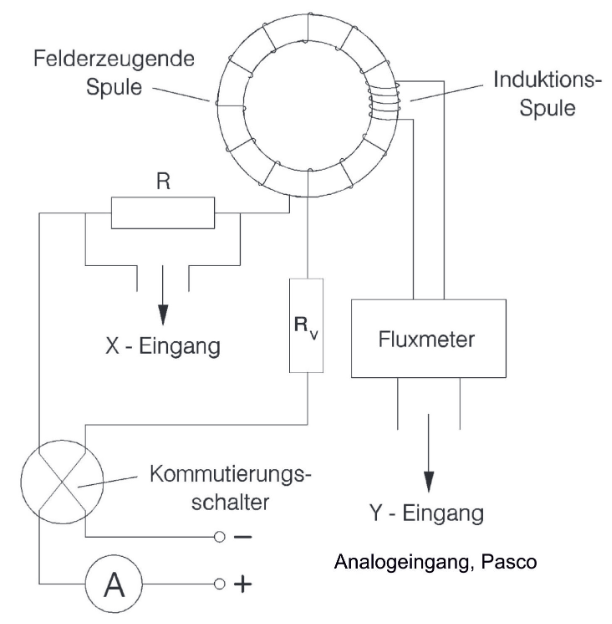
\includegraphics[width=0.9\linewidth]{ExperimentalSetup}
%        \caption{Setup for capturing hysteresis curves.
%        Channel X of the digital interface measures the current in the field-creating-coil $N_1$.
%        The ring core conducts the H-field.
%        The resulting B-field is measured by the induction-coil $N_2$.
%        The flux meter integrates analogously the voltage of the induction coil and its output is captured by
%        channel Y.
%        This enables to calculate the B-field at the induction-coil.}
        \caption{Aufbau zur Erfassung von Hysteresekurven.
        Eingang X der digitalen Schnittstelle misst die Spannung am Vorwiderstand und somit den Strom in der Feld-erzeugenden-Spule $N_1$.
        Der Ringkern leitet bzw. verstärkt das H-Feld.
        Dieses induziert Strom in der Induktionsspule $N_2$.
        Die Spannungsstöße von der Induktionsspule werden vom Fluxmeter analog integriert.
        Aus dem Wert, welcher von Eingang Y gemessen wird, kann das B-Feld berechnet werden.
        Bild aus~\cite{experimentManual}}
        \label{fig:ExperimentalSetup}
    \end{figure}
    
    Wir untersuchen die magnetischen Eigenschaften von vier Ringkernen, welche aus vier ausgewählten Materialien bestehen.
    Hierzu nutzen wir den Aufbau,
    wie er in Graphik~\ref{fig:ExperimentalSetup} dargestellt ist. 
    An der Feld-erzeugenden-Spule wird das Magnetfeld generiert.
    Die Stromstärke und damit die magnetische Feldstärke wird über den Spannungsabfall $U_{in}$ am Vorwiderstand
    bestimmt.
    Für den Eisenkern nutzen wir den Vorwiderstand $R = 0.20 \, \text{\Omega}$.
    Für die übrigen Kerne ist unsere maximale Stromstärke $I_{max} = 100 \, \text{mV}$, sodass wir den größeren
    Widerstand $R = (66.7 \pm 1.4) \, \text{\Omega}$ benutzen, um den Messbereich genauer aufzulösen.
    Das Feld, welches von der ersten Spule erzeugt wird, bestimmt sich über:
    \begin{align}
        \label{eq:CalculateHField}
        H = \frac{N_1}{\frac{\pi}{2}(d_i + d_o)R}U_{in}
    \end{align}
    Hier bezeichnet $d_i$ und $d_o$ den inneren bzw. \ äußeren Durchmesser des Ringkerns und $N_1$ ist die Windungszahl
    der Feld-erzeugenden-Spule.
    Der Querschnitt der Kerne wird hier als rechteckig angenommen.
    Für noch genauere Auswertung müssten noch die abgerundeten Ecken des realen Kerns mit einberechnet werden.
    
%    We have four ring cores of different materials.
%    To capture their magnetic properties we use the experimental setup shown in figure ~\ref{fig:ExperimentalSetup}. 
%    The external magnetic field is created by the first coil $N_1$.
%    We measure the current via the voltage drop $U_{in}$ at the first resistor.
%    Captured by the digital interface at Channel X.
%    For small currents we use $R = (66.7 \pm 1.4) \, \text{\Omega}$, else we use $R = 0.20 \, \text{\Omega}$.
%    The field created by the first coil can then be calculated with:
%    \begin{align}
%        \label{eq:CalculateHField}
%        H = \frac{N_1}{\frac{\pi}{2}(d_i + d_o)R}U_{in}
%    \end{align}
%    Where $d_i$ and $d_o$ are the inner and outer diameter of the ring core and $N_1$ is the winding number of the
%    field-creating-coil.
    
    Wie in Abbildung~\ref{fig:ExperimentalSetup} gezeigt, leitet der Ringkern das erzeugte Magnetfeld.
    Dies induziert einen Strom in der Induktionsspule mit Windungszahl $N_2$.
    Um das B-Feld zu bestimmen, benutzen wir ein Fluxmeter.
    Dieses integriert analog die Spannungsstöße der Induktionsspule.
    Der Wert wird als Spannungssignal ausgegeben,
    welches dann von der digitalen Schnittstelle auf Kanal Y aufgezeichnet wird.
    
    Die induzierte Spannung hängt von effektiven Querschnitt der Induktionsspule ab, welche vom Magnetfeld
    durchdrungen wird:
    \begin{align}
        \label{eq:EffectiveAreaOfInductionCoil}
        A_{eff} = \frac{1}{2} (d_o - d_i) h f
    \end{align}
    Wo $h$ die Höhe der Spule und $d_i$, $d_o$ der innere bzw.\ äußere Durchmesser sind.
    Ferner bezeichnet $f$ den Anteil von ferromagnetischem Material im Kern.
    Dieser Faktor muss berücksichtigt werden, da der zweite und dritte Kern aus \stripThickness dicken
    Fe-Ni-Bändern bestehen.
    Diese haben jeweils ein dünne Oxidschicht, sodass die effektive Füllmenge $f = 0.9$ ist.
    
%    The ring core conducts the field and induces a current in the second coil $N_2$.
%    To assess the conducted B-field, we use a flux-meter, which integrates analogously, the flux change of the second coil.
%    It's output is then captured by channel Y of the digital interface.
%    
%    The induced current depends on the effective area penetrated by the conducted field.
%    \begin{align}
%        \label{eq:EffectiveAreaOfInductionCoil}
%        A_{eff} = \frac{1}{2} (d_o - d_i) h f
%    \end{align}
%    Here $h$ is the height of the second coil and $d_o$ and $d_i$ the outer and inner diameter.
%    Furthermore $f$ is the effective percentage by which the ring core is filled with the ferromagnetic material.
%    This has to be account for since the second and third ring core consist of \stripThickness thin Fe-Ni-bands, which are coated by a oxid layer.
%    The effective fill percentage of these cores is $f = 90\%$.
    
    Aus dem Gesetz von Amp\´{e}re ergeben sich der vom Magnetfeld induzierte Strom.
    Das bedeutet, aus den integrierten Spannungsstößen, welche an Channel Y gemessen werden $U_{out}$, kann man
    auf das B-Feld zurückschließen:
    \begin{align}
        \label{eq:CalculateBField}
        B = \frac{\gamma_f}{N_2 A_{eff}} U_{F}
    \end{align}
    Hier bezeichnet $\gamma_f$ den Integrationsfaktor des Fluxmeters.
    
    Da das Fluxmeter analog integriert, gibt es eine unbestimmte Integrationskonstante, welche das Ausgangssignal $U_{out}$
    um einen konstanten Wert verschiebt.
    Diese Verschiebung wird korrigiert, indem wir die Daten zentrieren.
    Ferner entlädt sich der Kondensator im Fluxmeter mit der Zeit.
    Besonders für kleine Magnetfelder resultiert dies in einem konstanten Drift der Ausgangsspannung.
    Vergleiche hierzu Anhang~\ref{subsec:fluxDrift}.
    Für alle nachfolgend gezeigten Daten sind beide Effekte korrigiert.
    
%    Via Ampere's law you can calculate the induced current by the B-field.
%    Therefor with the integrated current measured at channel Y: $U_{out}$, you can infer the conducted field:
%    \begin{align}
%        \label{eq:CalculateBField} 
%        B = \frac{\gamma_f}{N_2 A_{eff}} U_{F}
%    \end{align}
%    Where $\gamma_f$ is the integration factor of the flux meter.
%    
%    Since the flux meter integrates analogously, there is an undetermined integration constants shifting the output
%    voltage $U_{out}$.
%    This shift is corrected by centering the data afterwards.
%    Furthermore the capacitor of the flux meter discharges naturally over time.
%    This results in a constant drift of the output voltage,
%    especially for small currents (compare section~\ref{subsec:fluxDrift}).
%    The following data is adjusted for both those effects.
    
    \section{Hysteresekurven}

    

    \subsection{Stahl ST37K}
    \label{subsec:steel}
    
%    \figExCoercivityRemanenceSteel{Hysteresis curve for steel ST37K\@.
%    Via linear regression the coercivity $H_C = \CoercivitySteel$ and remanence $B_R = \RemanenceSteel$ was accessed.
%    Furthermore with numerical integration the energy loss after equation~\eqref{eq:EnergyLoss} is $\xi = \HysteresisLossSteel$.
%    The saturation point was not reached.}
    
    \figExCoercivityRemanenceSteel{Hysteresekurve für Stahl ST37K\@.
    Mit linearer Regression wurde die Koerzitivfeldstärke $H_C = \CoercivitySteel$ und die
    Remanenz $B_R = \RemanenceSteel$ bestimmt. 
    Der Energieverlust kann durch numerische Integration bestimmt werden: $\xi = \HysteresisLossSteel$.
    Die Sättigung wurde nicht erreicht.
    }
    
%    We examined a ring core made of common construction steel ST37K\@.
%    The captured hysteresis curve can be seen in figure~\ref{fig:ExCoercivityRemanenceSteel}.
%    To get the coercivity and remanence we apply linear regression around the H- and B-axis respectively.
%    Since the the curve is in proximity of the intersection linear.
    
    Als erstes betrachten wir einen Ringkern, welcher aus handelsüblichen Baustahl ST37K besteht. %// TODO
    Die erfasste Hysteresekurve ist in Abbildung~\ref{fig:ExCoercivityRemanenceSteel} dargestellt.
    Um die Koerzitivfeldstärke und Remanenz zu erhalten, wenden wir lineare Regression an, da die Kurve in der Nähe
    der Schnittpunkte linear ist.
    
    \begin{align*}
        H_C &= \CoercivitySteel \\
        B_R &= \RemanenceSteel
    \end{align*}
%    The error was inferred by the statistical scattering of the data points around the linear regression.
%    Please be aware that this approach only reflects statistical errors.
%    In our measurements we have a large amount of systematical errors, due to the fact that magnetic hysteresis is
%    highly dependent on the geometry of the used ring cores. 
%    Moreover depending on the manufacturing process, the grain size varies, which greatly affects the permeability of
%    the material.
%    To make our results reproducible, a far greater control over these factors would be required.
%    Because this paper is more concerned with qualitative results, all quantitative results only really apply for the
%    local setup used by us.
    
    Der Fehler wurde aus der statistischen Streuung der Datenpunkte bestimmt.
    Es ist zu beachten, dieser Ansatz gibt nur statistische Fehler wieder.
    Unsere Messergebnisse weisen aber große systematische Unsicherheiten auf, welche sie nicht reproduzierbar machen.
    Magnetische Hysterese hängt stark von der Geometrie und dem Material selbst ab.
    Je nach Herstellungsprozess variiert die Korngröße, was die magnetische Permeabilität des Materials stark beeinflusst.
    So ist die Angabe der Norm ST37K nicht aussagekräftig genug.
    Sie bestimmt nicht den genauen Herstellungsprozess.
    Wir wollen in diesem Paper nicht, magnetische Werte für ein bestimmtes Material veröffentlichen.
    Wir wollen eine Methode vorstellen, wie die magnetischen Parameter für ein gegebenes Material gemessen werden können.
    Wenn man reproduzierbare Ergebnisse erhalten möchte, dann muss man darauf achten, die Geometrie und Herstellung
    des Materials genau zu kontrollieren.
    Das bedeutet alle hier vorgestellten Werte, gelten nur auf die von uns verwendeten Ringkerne.
    Trotzdem kann die Methode auf jedes beliebige Material angewandt werden.
    
%    The energy loss was calculated by numerical integrating the curve and applying equation~\eqref{eq:EnergyLoss}:
    Der Energieverlust kann mit Hilfe von Gleichung~\eqref{eq:EnergyLoss} bestimmt werden.
    \begin{align*}
        \xi = \HysteresisLossSteel
    \end{align*}
    %Similarly the error was determined by the statistical scattering of the data points.
    Analog zu Oben, wurde der Fehler aus der statistischen Streuung der Datenpunkte bestimmt.
    Es wurde hierzu eine minimale und maximale Fläche numerisch in die Kurve gelegt.
    
%    To determine the area under the curve we also tried the alternative approach of cutting out paper-curves and
%    weighing the cutout.
%    This turned out to be inaccurate.
%    See appendix~\ref{subsec:ManualIntegration} for the results.
    Um das Integral zu bestimmen versuchten wir neben der nummerischen Methode auch den Ansatz, den Graphen auszudrucken
    die Kurve auszuschneiden und dann zu wiegen.
    Dies Methode hat sich als unzuverlässig herausgestellt.
    Die Ergebnisse sind im Anhang~\ref{subsec:ManualIntegration} aufgelistet.
    
    \subsubsection{Irreverisbilität der Hysterese}
    
%    \figExIrreversibilitySteel{Hysteresis curve for ST37K.
%    By briefly changing direction of the applyied H-field a hysteresis-branch is formed.
%    This shows the time dependence of ferromagnetical materials. 
%    It can be explained via Weiss domains (c.f. section~\ref{sec:Theory})}
    \figExIrreversibilitySteel{Hysteresekurve für Stahl ST37K.
    Wenn man im Bereich, wo das H-Feld kontinuierlich verringert wird,
    dieses kurzzeitig wieder erhöht, dann formt sich ein Ast in der Hysteresekurve.
    Die Magnetisierung geht nicht zu ihrem voherigen Wert zurück sondern ist schwächer.
    Dies zeigt, dass die Magnetisierung von der Vergangenheit des Materials abhängt.}
    
%    As stated in section~\ref{sec:Theory}, the hysteresis curve depends on the magnetization history
%    of the material. 
%    This effect can be revealed by briefly flipping the direction of the external H-field.
%    Compare figure~\ref{fig:ExIrreversibilitySteel} where after changing the field direction a branch in the curve
%    is formed.
%    The magnetization does not return to its previous state, instead it is weaker.
%    
%    This is due to the fact, that moving the boundaries over the lattice defects costs energy $E_{def}$.
%    As you can see in figure~\ref{fig:ExIrreversibilitySteel} if we start in a polarized state
%    and now remove the H-field, the magnetic moments scatter, to reach an energetic more favorable state.
%    We get energy $E_{moments}$.
%    So the energy change is:
    
    Wie in Abschnitt~\ref{sec:Theory} beschrieben, hängt die Hysterese von der Magnetesierungsvergangenheit
    des Materials ab.
    Dieser Effekt lässt sich dadurch zeigen in dem man eine kurze Richtungsänderung am äußeren H-Feld vornimmt.
    D.h.\ befinden wir uns gerade in dem Bereich, wo wir kontinuierlich das H-Feld verringern, dann erhöhen wir es
    kurzfristig wieder.
    Entgegen der Erwartung kehrt die Magnetisierung dann nicht in ihren vorherigen Zustand zurück, sonder sie
    wird schwächer.
    Es bildet sich ein Ast in der Hysteresekurve aus.
    
    Dies ist darauf zurückzuführen, dass die Bewegung der Block-Wände über die Gitterdefekte Energie $E_{def}$ kostet.
    Vergleichen Sie hierzu Abbildung~\ref{fig:ExIrreversibilitySteel}.
    Wir beginnen in einem magnetisierten Zustand.
    Die magnetischen Momente sind ausgerichtet.
    Erniedrigen wir nun das H-Feld, dann gehen die Dipolmomente in einen ungeordneten Zustand über.
    Dieser ist energetisch günstiger.
    Wir erhalten also Energie $E_{moments}$.
    Das bedeutet die Gesamtenergieänderung ist:
    
    \begin{align*}
        \Delta E &= E_{moments} - E_{def}
    \end{align*}
%    If we now increase the H-field and polarize the material again, we have to again put in this energy $E_{moments}$.
%    But it still costs energy to move the boundaries between the weiss domains over defects $E_{def}$.
%    So the energy change is:
    
    Wenn wir nun das H-Feld kurzzeitig wieder erhöhen und das Material wieder magnetisieren, dann müssen wir die
    `Umordnungsenergie' $E_{moments}$ wieder hineinstecken.
    Es kostet aber immer noch Energie $E_{def}$ die Blockwände über die Defekte zu bewegen.
    Somit ist die Gesamtänderung:
    
    \begin{align*}
        \Delta E &= - E_{moments} - E_{def}
    \end{align*}
%    But this means we have overall lost energy, thus the polarisation has to be weaker.
%    
%    This fact holds also true if we traverse the whole hysteresis loop.
%    We have determined this exact energetic loss in the previous section to be:
    
    Aber dies bedeutet, wir haben insgesamt Energie verloren.
    Somit muss die Magnetisierung schwächer sein.
    
    Dies gilt auch, wenn wir die gesamte Hystereseschleife durchlaufen.
    Wir haben diesen Energieverlust schon im vorherigen Abschnitt bestimmt:
    
    \begin{align*}
        \xi = \HysteresisLossSteel
    \end{align*}
    
    \subsubsection{Entmagnetisierung}
    
%    \figExDemagnetizationSteel{Hysteresis curve for steel ST37K.
%    The steel was demagnetized by continously flipping and decreasing the applied H-field.
%    Because of energy losses, the magnetization gets weaker every time you reverse the H-field.
%    In the inlet can be seen, we did not exactly reach a state of complete demagnitization.
%    This is due to the constraint, that we did control the H-field manually.}
    \figExDemagnetizationSteel{Hysteresekurve von Stahl ST37K.
    Der Stahl wurde entmagnetisiert, indem wiederholt das H-Feld umgekehrt und verringert wurde.
    Auf Grund von Energieverlusten nimmt die Magnetisierung immerweiter ab.
    In der Vergrößerung ist zu erkennen, dass wir nicht exakt den Zustand vollständiger Entmagnetisierung
    erricht haben.
    Dies liegt daran, dass wir das H-Feld manuell gesteuert haben.
    }
    
%    As shown in the previous section, after you reverse the rate of change of the external field, the magnetisation
%    is weaker as in the previous state.
%    You can use this fact to demagnetize the material.
%    This was achieved by periodically flipping the H-field and decreasing its strength each step,
%    The magnetic moments of the weiss domains get more and more disordered, until no remanence-field is left.
%    The lowest energetic state is reached.
%    
%    As you can see in figure~\ref{fig:ExDemagnetizationSteel} we did not reach the state of demagnetization perfectly.
%    This is due the fact, that we controlled the H-field manually.
    
    Wie im vorherigen Abschnitt gezeigt, nach der kurzzeitigen Umkehr der Änderungsrate des H-Feldes
    ist die Magnetisierung schwächer als im vorherigen Zustand.
    Dieser Effekt kann ausgenutzt werden um das Material zu entmagnetisieren.
    Hierzu haben wir periodisch das H-Feld umgekehrt.
    Nach jedem Schritt nimmt die Magnetisierung ab.
    Die Weiss-Bezirke nehmen Schritt für Schritt einen immer ungeordneteren Zustand ein, solange bis
    kein Remanenzfeld mehr übrig bleibt.
    Der Zustand niedrigster Energie ist erreicht und das Material ist entmagnetisiert.
    
    Wie Sie in Abbildung~\ref{fig:ExDemagnetizationSteel} sehen können, haben wir
    keinen komplett entmagnetisierten Zustand erreicht.
    Dies liegt daran, dass wir das H-Feld manuell steuerten, und es somit nicht exakt einstellen konnten.


    \subsection{PERMENORM 5000 H2 Fe-Ni-Legierung}

%    \figExSaturationFeNiHTwo{Captured hysteresis curve for \stripThickness thick Fe-Ni `PERMENOR 5000 H2' strips.
%    To test if we have reached the saturation, a line was fitted at the end of the curve.
%    The determined permeablity is $\mu = \SaturationPermeabilityFeNiHTwo \mu_0$.
%    This means we have not reached the saturation point, where the permability should be $\mu = \mu_0$.}

    \figExSaturationFeNiHTwo{
        Hysteresekurve für \stripThickness dicke Fe-Ni-`PERMENORM 5000 H2'-Bänder.
        Um zu prüfen, ob wir die Sättigung erreicht haben, wurde die Steigung am Ende der
        Hysteresekurve ermittelt.
        Die Permeablilität beträgt $\mu = \SaturationPermeabilityFeNiZ \mu_0$.
        Folglich haben wir nicht den Sättigungspunkt erreicht.
        Ab diesem sollte die Permeabilität gleich
        der Vakuumspermeabilität sein $\mu = \mu_0$.
    }


%    The second core, which we examined, consisted of the industrial Fe-Ni-Alloy `PERMENORM 5000 H2'.
%    It is constructed out of \stripThickness thin metal bands.
%    The thickness of the metal strips greatly influences the magnetic properties of the material~\cite{feniDatasheet}.
%    For the measurement we used the former setup but with the additional resistor $R = (66.7 \pm 1.4) \, \text{\Omega}$,
%    to have a higher resolution, since we had a maximum current of $I = 100mA$.
%    
%    By applying linear regression, we determine the coercivity and remanence field.
%    Furthermore via numerical integration we calculated the energy loss.

    Der zweiter Kern, welchen wir untersuchten, bestand aus der industriellen Fe-Ni-Legierung `PERMENORM 5000 H2'.
    Er ist aus \stripThickness dicken Metallbändern aufgebaut.
    Die Dicke hat einen großen Einfluss auf die magnetischen Eingenschaften des Materials, vgl. \cite{feniDatasheet}.
    Für die Messung benutzen wir den vorherigen Aufbau, jedoch mit dem zusätzlichen Vorwiderstand
    $R = (66.7 \pm 1.4) \, \text{\Omega}$.
    Hiermit können wir die Stromstärke besser auflösen, da der Maximalstrom für die Spulen nur
    $I = 100\,\text{mA}$ betrug.

    Mit Hilfe von lineare Regression konnte die Koerzitivfeldstärke und das Remanenzfeld bestimmt werden.
    Ferner mit Hilfe von nummerischer Integration konnte der Energieverlust bestimmt werden:

    \begin{align*}
        H_C &= \CoercivityFeNiHTwo \\
        B_R &= \RemanenceFeNiHTwo \\
        \xi &= \HysteresisLossFeNiHTwo
    \end{align*}

%    As mentioned these values have a high degree of systematical uncertainty.
%    We can compare them with the datasheet of the manufacturer~\cite{feniDatasheet}.
%    The coercivity for 0.35mm thick `PERMENORM 5000 H2' strips is:
    Wie bereits erwähnt, besitzen die angegebenen Werte ein hohes Maß an systematischen Fehlern.
    Wir können die Werte mit dem Datenblatt des Herstellers~\cite{feniDatasheet} vergleichen.
    Die Koerzitivfeldstärke für $0.35\,\text{mm}$ dicke `PERMENORM 5000 H2'-Bänder beträgt:
    \begin{align*}
        H_C &= 3 \ A/m
    \end{align*}
%    Our results are in the same order but do not agree.
%    This is due to the fact that there is no datasheet for \stripThickness thick strips publicly available.
%    But the thickness as a high impact.
%    Further the values of the datasheet have a large uncertainty themself.
%    
%    As mentioned in section~\ref{sec:Theory} there is a point where the applied H-field is great enough,
%    so all magnetic moments are aligned.
%    At this saturation point there is no amplification of the magnetic field.
%    The slope of the hysteresis curve is $\mu_0$.
%    
%    To test, weather we have reached the saturation point, we fit a line at the end of the hysteresis
%    curve as shown in figure~\ref{fig:ExSaturationFe-Ni H2}.
%    The field and the permeability are:

    Unsere Ergebnisse befinden sich in der gleichen Größenordnung aber stimmen nicht überein.
    Dies liegt daran, dass dies die Angabe für $0.35\,\text{mm}$ dicke Bänder sind.
    Die Angaben für \stripThickness dicke Bänder sind leider nicht öffentlich zugänglich.
    Die Dicke des Bandes hat aber einen sehr großen Einfluss auf die Hysterese-Eigenschaften.
    Ferner beachte man auch, dass die Herstellerangaben selbst mit einer großen Unsicherheit behaftet sind.

    Wie im Abschnitt~\ref{sec:Theory} erwähnt, gibt es einen Punkt an dem das äußere H-Feld stark genug ist,
    sodass all magnetischen Momente ausgerichtet sind.
    Ab diesem Sättigungspunkt wird das äußere Magnetfeld nicht mehr verstärkt.
    Die Steigung der Hysteresekurve ist dann $\mu_0 = 1.25663706212\cdot 10^{-6} \, \mathrm{N/A^2}$~\cite{codata}.

    Um nun zu testen, ob wir den Sättigungspunkt erreicht haben, bestimmen wir die Steigung an den Enden der
    Hysteresekurve.
    Wir führen hierzu lineare Regression durch, wie in Abbildung~\ref{fig:ExSaturationFe-Ni H2} gezeigt ist.
    Die Permeabilität und das Magnetfeld sind:

    \begin{align*}
        B_S &= \SaturationFeNiHTwo \\
        \mu &= \SaturationPermeabilityFeNiHTwo \ \mu_0
    \end{align*}
%    Obviously we have not reached the saturation point.
%    The datasheet confirms this.
%    It states, the saturation magnetization at $H = 40 \ kA/m$ to be:

    Offensichtlich haben wir nicht den Sättigungspunkt erreicht, da die Permeabilität um drei Ordnungen größer als
    die Vakuumspermeabilität ist.
    Das Datenblatt bestätigt dies.
    Hiernach ist die Sättigung bei einer externen Feldstärke von $H = 40 \, \text{kA/m}$ erreicht.
    Das Sättigungsfeld ist:

    \begin{align*}
        B_S &= 1.60 \ T
    \end{align*}
%    In our measurement we did not reach such a strong H-field.
%    The coils did not withstand such high currents.
%    A more robust setup would be required.
%    
%    If we compare this Fe-Ni-Alloy to the previous core out of steel ST37K, we see the alloy as a much lower coercivity and subsequent energy
%    loss.
%    This makes it ideal for applications in current transformers and magnetic shielding~\cite{feniDatasheet}.

    In unserer Messung haben wir keine so starken H-Felder erreicht.
    Die genutzten Spulen waren auf keine so große Ströme ausgelegt.
    Es benötigt einen robusteren Aufbau, um die Sättigung zu bestimmen.

    Wenn wir die Fe-Ni-Legierung zum vorherigen Kern aus Stahl ST37K vergleichen, stellen wir fest, dass die Legierung eine
    deutlich geringere Koerzitivfeldstärke und damit geringeren Energieverlust aufweist.
    Dies macht sie ideal für Anwendungen in Transformatoren und magnetischen Abschirmungen~\cite{feniDatasheet}.

    \subsection{PERMENORM 5000 Z Fe-Ni-Legierung}

%    \figExFeNiZ{Hysteresis curve for the Fe-Ni-Alloy `PERMENORM 5000 Z'.
%    It also consists of \stripThickness thin strips.
%    The maximum permeablity is high, while the coercivity is still low $H_C = \CoercivityFeNiZ $.
%    The material can also be used for transformer cores, magnetic shielding and current and positioning 
%    sensors~\cite{feniDatasheet}.
%    }
    \figExFeNiZ{
        Hysteresekurve für \stripThickness dicke Fe-Ni-`PERMENORM 5000 Z'-Bänder.
        Die maximale Permeabilität (maximale Steigung) ist hoch, während die Koerzitivfeldstärke gering ist
        $H_C = \CoercivityFeNiZ$.
        Das Material kann für Transformatorkerne, magnetische Abschirmungen und Strom- bzw. Positionssensoren benutzt werden~\cite{feniDatasheet}.
    }

%    The third core consisted of the Fe-Ni-Alloy `PERMENORM 5000 Z'.
%    It is also constructed out of \stripThickness thin Fe-Ni-strips.
%    Analogously to the coercivity, remanence and energy loss was calculated:
    Der dritte Kern bestand aus der Eisen-Nickel-Legierung `PERMENORM 5000 Z'.
    Er ist auch aus \stripThickness dicken Fe-Ni-Bändern aufgebaut.
    Analog wurde Koerzitivfeldstärke, Remanenz und Energieverlust bestimmt:

    \begin{align*}
        H_C &= \CoercivityFeNiZ \\
        B_R &= \RemanenceFeNiZ \\
        \xi &= \HysteresisLossFeNiZ
    \end{align*}

%    Also to test weather we have reached the saturation point, we determined the permeability at the end of the curve:

    Um zu überprüfen, ob wir die Sättigung erreicht haben, wurde die Permeabilität am Ende der Kurve bestimmt:

    \begin{align*}
        B_S &= \SaturationFeNiZ \\
        \mu &= \SaturationPermeabilityFeNiZ \ \mu_0
    \end{align*}
%    Obviously the saturation point was also not reached.
%    There is no datasheet publicly available to verify these results.
%    
%    Since the maximum permeability is quite high as seen in figure~\ref{fig:ExFe-Ni Z} and the coercivity is still
%    low, the material can also be used in transformers, magnetic shields and current and positioning sensors~\cite{feniDatasheet}.

    Auch hier wurde die Sättigung nicht erreicht.
    Es ist kein öffentlich zugängliches Datenblatt vorhanden, um die Ergebnisse zu überprüfen.

    Wie in Abbildung~\ref{fig:ExFe-Ni Z} zu sehen ist, ist die maximale Permeabilität recht hoch, während
    die Koerzitivfeldstärke gering ist.
    Damit kann das Material in Transformatoren, magnetischen Abschirmungen sowie Strom- und Positionssensoren genutzt werden.



    \subsection{Holz als Referenz für einen Paramagneten}
    
%    \figMessreiheKernFourOneEightTwoRWood{Paramagnetic amplification by a ring core consisting of wood.
%    Via regression the susceptibility was calculated: $\chi &= \WoodMagneticSusceptibility$.
%    The susceptibility is very high, which makes the material superparamagnetic.
%    Probably the core does not consist of wood after all.
%    We can not verify this, because we did not build the core.}
    \figMessreiheKernFourOneEightTwoRWood{
    Paramagnetische Verstärkung durch einen aus Holz bestehenden Ringkern.
    Durch Regression wurde die Suszeptibilität berechnet: $\chi = \WoodMagneticSusceptibility$.
    Die Suszeptibilität ist sehr hoch, so lässt sich das Material als superparamagnetisch einstufen. 
    Die Abweichung könnte auf Grund von unbeachteten Widerständen im Aufbau kommen,
    denn die gemessenen Spannungsstöße sind um einen Faktor 100 kleiner als bei den feromagnetischen Materialien.
    Hier zeigen sich die Grenzen des Aufbaues auf.
    }
    
%    To compare our results, we examined a core made of wood as an example for a paramagnetic material.
%    
%    Paramagnetism is caused by magnetic moments of unpaired spins\cite{gerth}.
%    Similarly to ferromagnetism these magnetic moments do align, when an external H-field is applied,
%    and thus amplifying it.
%    But in contrast to ferromagnetism, no weiss domains are formed, meaning the polarisation does not depend
%    on the history.
%    Furthermore the amplification by paramagnets is weak.
%    The susceptibility is generally in the order of:
    
    Um unsere Ergebnisse zu vergleichen, haben wir einen Holzkern als Beispiel für ein paramagnetisches 
    Material untersucht.
    
    Paramagnetismus wird durch die magnetischen Dipolmomente von Atomspins verursacht.
    Analog zum Ferromagnetismus, richten sich die magnetischen Momente aus, wenn ein äußeres H-Feld angelegt wird.
    Aber im Gegensatz zu Ferromagnetismus, kuppeln benachbarte Spins nicht aneinander.
    Es kommt zu keiner Ausbildung von Weiss-Bezirken.
    Somit hängt die Magnetisierung nicht von der Vergangenheit des Materials ab und es kommt zu keiner Hysterese.
    Ferner ist die Verstärkung durch Paramagneten schwach.
    Die magnetische Suszeptibilität liegt im Allgemeinen in der Größenordnung von~\cite{gerth}:
    
    \begin{align*}
        \chi  &\sim 10^{-5}
    \end{align*}
    
%    As you can see in figure~\ref{fig:Messreihe_Kern4_18_2_RWood} in our measurements, no hysteresis curve was formed.
%    This shows the examined material is paramagnetic.
%    The susceptibility was determined by fitting a line in the data points.
    
    Wie in Abbildung~\ref{fig:Messreihe_Kern4_18_2_RWood} gesehen werden kann, bildet sich keine Hysteresekurve aus.
    Dies zeigt, das untersuchte Material ist paramagnetisch.
    Die Suszeptibilität wurde bestimmt in dem eine Gerade in die Daten gefittet wurde:
    
    \begin{align*}
        \chi &= \frac{\mu}{\mu_0} - 1 = \WoodMagneticSusceptibility
    \end{align*}
    
%    The measured susceptibility is much higher as would be expected from a paramagnetic material.
%    In fact the susceptibility is great enough, that the material can be considered superparamagnetic.
%    Probably the core did not solely consist of wood.
%    There has to be another material part of the core.
%    Maybe it is a ferromagnet above the curie temperature, since they exhibit superparamagnetic behaviour.
%    We can not verify these theories, because we did not build the cores.
%    A closer inspection would be required.
    
    Die gemessene Suszeptibilität ist deutlich höher als man von einem paramagnetischen Material erwarten würde.
    Tatsächlich ist die Suszeptibilität so groß, dass das Material als superparamagnetisch betrachtet werden kann.
    Es gibt verschiedene Erklärungsmöglichkeiten für diese Abweichung.
    Zum einen könnte beim Messaufbau ein systematischer Fehler vorliegen.
    So sind die Stromstöße, welche vom Fluxmeter gemessen werden um zwei Größenordnungen kleiner als bei den
    ferromagnetischen Kernen.
    Nicht beachtete Verluste, könnten die Abweichung verursachen.
    Eine weitere Erklärungsmöglichkeit wäre, dass im Kern ein weiteres Material neben Holz verbaut ist.
    Es könnte sich um ein ferromagnetisches Material oberhalb der Curie-Temperatur handeln.
    Diese weisen superparamagnetisches Verhalten auf.
    Es wäre eine genaue Inspektion des Aufbaus erforderlich, um diese Spekulationen zu bestätigen.
    
    
    \section{Fazit}
    
%    We wanted to examine the characteristic hysteresis curve for ferromagnetic materials.
%    For this we used a setup of two coils.
%    The first on creates the H-field.
%    This field is then conducted by the ferromagnetic core, and induces a current in the second coil.
%    Via analog integration we can determine the conducted B-field.
%    
%    For three ferromagnetic materials we tested this setup.
%    For steel ST37K we captured the hysteresis curve and via linear regression we calculated the coercivity
%    $H_C = \CoercivitySteel$ and the remanence field $B_R = \RemanenceSteel$.
%    Furthermore with numerical integration we can calculate the energy loss of traversing on hysteresis loop:
%    $\xi = \HysteresisLossSteel$.
%    The irreversibility of hysteresis was shown by briefly flipping the direction of the H-field.
%    This was then applied to demagnetize the steel core, by continuously flipping the direction till now remanence-field
%    was left.
%    
%    We repeated this process for the industrial Fe-Ni alloy `PERMENORM 5000 H2'.
%    It is a soft magnetic material.
%    It coercivity was measured to be $H_C = \CoercivityFeNiHTwo$, the remanence $B_R = \RemanenceFeNiHTwo$
%    and the energy loss $\xi = \HysteresisLossFeNiHTwo$.
%    We tested weather we have reached the saturation point by applying a linear fit at the end of the curve.
%    The measured slope was $\mu = \SaturationPermeabilityFeNiHTwo \ \mu_0$, which means we did not reach saturation.
%    Far greater H-Fields would be required.
%    
%    For the magnetically harder alloy `PERMENORM 5000 Z' the characteristic properties were:
%    $H_C = \CoercivityFeNiZ$, $B_R = \RemanenceFeNiZ$ and $\xi = \HysteresisLossFeNiZ$.
%    Here we also did not reach the saturation point.
%    
%    Lastly a paramagnetic core was examined.
%    It's susceptibility was measured as $\chi = \WoodMagneticSusceptibility$.
%    This would make the core superparamagnetic.
%    
%    Please note all stated values above only really apply for our local setups. 
%    Magnetic hysteresis is greatly dependent on the manufacturing process of the material and it's exact geometry.
%    In this paper we wanted to show the principle on how to capture hysteresis and
%    how to extract the important magnetic properties.
%    For more general applicable data, greater control over the material and geometry would be necessary.
    
    Wir stellen eine Methode vor, um charakteristische Eigenschaften von ferromagnetischen Materialien zu untersuchen.
    Hierzu haben wir einen Aufbau mit zwei Spulen verwendet.
    Die erste Spule erzeugt das H-Feld.
    Dieses Feld wird dann durch den ferromagnetischen Kern geleitet bzw.\ verstärkt und induziert in der zweiten Spule
    einen Strom.
    Durch analoge Integration können wir dann das verstärkte B-Feld bestimmen.
    
    Für drei ferromagnetische Materialien haben wir diesen Aufbau getestet.
    Für Stahl ST37K haben wir die Hysteresekurve aufgenommen und mit linearer Regression die
    Koerzitivfeldstärke $H_C = \CoercivitySteel$ und das Remanenzfeld $B_R = \RemanenceSteel$
    bestimmt.
    Ferner können wir durch nummerische Integration den Energieverlust beim Durchlaufen einer
    Hystereseschleife berechnen: $\xi = \HysteresisLossSteel$.
    Die Irreverisbilität der Hysterese wurde durch eine kurze Umkehrung der Richtung des H-Feldes nachgewiesen.
    Dies wurde dann zur Entmagnetisierung des Stahlkerns verwendet.
    Hierzu wurde das H-Feld wiederholt umgekehrt, bis keine Remanenz übrig bleibt.
    
    Wir haben dieses Verfahren für die industrielle Fe-Ni-Legierung `PERMENORM 5000 H2' wiederholt.
    Der Kern bestand aus \stripThickness dicken Fe-Ni-Bändern.
    Es handelt sich hier um ein magnetisch weiches Material, denn die Koerzitivfeldstärke betrug
    $H_C = \CoercivityFeNiHTwo$, die Remanenz $B_R = \RemanenceFeNiHTwo$ und der Energieverlust
    $\xi = \HysteresisLossFeNiHTwo$.
    Wir haben geprüft, ob wir den Sättigungspunkt erreicht haben, indem wir eine Gerade in das Ende der Hysteresekurve
    gefittet haben.
    Die Permeabilität war $\mu = \SaturationPermeabilityFeNiHTwo \ \mu_0$, was bedeutet, dass
    wir die Sättigung nicht erreicht haben.
    Hierfür benötigt man deutlich größere H-Felder.
    
    Für die magnetisch härtere Legierung `PERMENORM 5000 Z' waren die charakteristische Parameter:
    $H_C = \CoercivityFeNiZ$, $B_R = \RemanenceFeNiZ$ und $\xi = \HysteresisLossFeNiZ$.
    Auch hier haben wir den Sättigungspunkt nicht erreicht.
    
    Zum Schluss wurde ein paramagnetischer Kern untersucht.
    Seine Suszeptibilität wurde bestimmt: $\chi = \WoodMagneticSusceptibility$.
    Dies würde den Kern superparamagnetisch machen.
    Dies zeigt die Grenze des Aufbaus auf, da er für sehr schwache Magnetfelder er eine systematische 
    Abweichung zeigt.
    
    Es ist zu beachten, dass alle oben genannten Werte nur für die von uns verwendeten Kerne gelten.
    Die hier angegebenen Werte sind nicht reproduzierbar.
    Hysterese hängt stark von der Geometrie und Herstellungsprozess des Materials da.
    In diesem Paper wollen wir vorstellen, wie man die charakteristischen Größen für ein gegebenes
    ferromagnetisches Material bestimmt.
    Für allgemein gültige Daten ist deutlich bessere Kontrolle über Material und Geometrie erforderlich.
    
    
    %FF: Angabe der verwendeten Literatur mit Quellennachweis.
    \begin{thebibliography}{}    %so wird das Literaturverzeichnis erstellt
        \bibitem{gerth} Meschede, Dieter, Gerthsen Physik, 25. Auflage, Springer-Verlag, Berlin, 2015
        \bibitem{feymanLecturesWeisDomains}  Feynman, Richard P.; Robert B. Leighton; Matthew Sands (1963).
        The Feynman Lectures on Physics. Volume 2.
        \bibitem{feniDatasheet} Datasheet PERMENORM 5000 H2: \url{https://vacuumschmelze.de/03_Documents/Brochures/PERMENORM%205000%20V5%20H2%20Strip.pdf},
        abgerufen am 02.10.2023
        \bibitem{codata} CODATA Recommended Values. National Institute of Standards and Technology, abgerufen am 4.10.2023
        \bibitem{experimentManual} Physikalisches Grundpraktikum, Universitüt Würzburg, Modul C1, Versuch 39, Hysterese von verschiedenen ferromagnetischen Materialien, 2021
    \end{thebibliography}
    
    %\clearpage
    
    \section{Anhang}

    \subsection{Flux drift}
    \label{subsec:fluxDrift}

%    \figNoDriftRemovalWood{Captured magnetic curve for wood core.
%    The data is centered but the flux drift caused by the flux meter was not accounted for.
%    This is due to the capacitor of the flux meter discharges over time.}
    \figNoDriftRemovalWood{
    Aufgezeichnete B-H-Graphen für einen Holzkern.
    Die Daten wurden zentriert aber der Fluxdrift wurde nicht mit einberechnet.
    Da sich der Kondensator im Fluxmeter mit der Zeit entlädt,
    scheint es, als würde sich das B-Feld mit der Zeit stärker werden.
    In allen anderen gezeigten Datensätzen wurde dieser Effekt berücksichtigt.
    }
    
%    To capture the induced B-field we use a flux meter.
%    It integrates the voltage surges of the coil and outputs an analog signal.
%    For the integration it uses a capacitor.
%    But the capacitor naturally discharges overtime.
%    This results in the flux drift, where the B-field seemingly increases over time 
%    as can be seen in figure~\ref{fig:NoDriftRemovalWood}.
%    To account for this effect the B-field at the start $B_s$ and at the end $B_e$ are used to calculate the shift
%    over time.
    Zur Erfassung des induzierten B-Feldes verwenden wir ein Fluxmeter.
    Es integriert die Spannungsstöße der Spule und gibt ein Spannungssignal über den analogen Ausgang zurück.
    Für die Integration benutzt es einen Kondensator.
    Dieser Kondensator entlädt sich mit der Zeit.
    Dies führt zu einem Fluxdrift, wo das B-Feld sich scheinbar mit der Zeit erhöht, wie 
    in Abbildung~\ref{fig:NoDriftRemovalWood} zu sehen ist.
    Um diesen Effekt zu berücksichtigen, wird das Feld am Anfang $B_s$ und am Ende $B_e$ benutzt umd die
    zeitliche Veränderung zu berechnen:
    \begin{align*}
        \dot{B}_{drift} &= \frac{B_e - B_a}{\Delta t}
    \end{align*}
%    All data points are then offset by this factor.
    Alle Datenpunkte werden dann um diesen Faktor verschoben.
    
    \subsection{Integration mit Papierausschnitt}
    \label{subsec:ManualIntegration}
    
%    To determine the energy loss of one hysteresis loop the area under the curve has to be determined.
%    We used the numerical approach, by fitting a spline through the curve and then integrating that spline.
%    An alternative approach we tried, is to printout the hysteresis curves.
%    Then cutting out the curve, which we then weighted with a precision scale.
%    The energy loss for the steel core determined by this method is:
    Um den Energieverlust einer Hystereseschleife zu bestimmen, muss die Fläche unter der Kurve ermittelt werden.
    Wir verwendeten den numerischen Ansatz, indem wir eine Spline durch die Daten zogen
    und dann die Fläche unter der Spline bestimmten.
    Ein alternativer Ansatz, welchen wir versuchten, bestand darin, den Graphen der Hysteresekurve auszudrucken.
    Dann schnitten wir die Kurve aus, und wiegten diese mit Hilfe einer Präzisionswaage.
    Der mit dieser Methode ermittelte Energieverlust für den Stahlkern beträgt:
    \begin{align*}
        \xi &= (0.2759 \pm 0.0013) \, \text{J/kg}
    \end{align*}
%    Comparing that to the numerical result:
    Verglichen mit dem numerischen Ergebnis:
    \begin{align*}
        \xi &= \HysteresisLossSteel
    \end{align*}
    Diese Werte stimmen innerhalb ihrer Fehler nicht überein.
    Dies liegt daran, dass für der Fehler der Ausschneide-Methode nur der Fehler der Waage herangezogen werden konnte,
    da der eigentlich dominate manuelle Fehler des Ausschneidens nicht vernünftig abgeschätzt werden kann.
%    These values do not agree with respect to their uncertainties.
%    This is due to the fact, that for the error of the cutout-method only the scale uncertainty was used.
%    Since the dominating manual error of the cutout cannot reasonably be determined.
    
    Analog ist der Wert für die Fe-Ni-Legierung `PERMENORM 5000 H2':
%    Analogously the value for the Fe-Ni-Alloy `PERMENORM 5000 H2' is:
    \begin{align*}
        \xi &= (2.749 \pm 0.017) \cdot 10^{-3} \, \text{J/kg}
    \end{align*}
    Hierzu im Vergleich das numerische Ergebnis:
%    In comparison the numerical result:
    \begin{align*}
        \xi &= \HysteresisLossFeNiHTwo
    \end{align*}
%    Since the cutout method has such high unreliability, those results were not shown in the main paper.
    
    Da die Ausschneide-Methode so eine hohe Unzuverlässigkeit aufweist, wurden diese Ergebnisse im eigentlichen Paper
    nicht verwendet.
    
    
\end{document}